\documentclass{tudelft-report}

%% Set up the bibliography
\usepackage{biblatex}
\addbibresource{report.bib}

%% Additional packages and commands
\usepackage{parskip}
\setlist{itemsep=-2pt} % Reducing white space in lists slightly
\renewcommand{\deg}{\si{\degree}\xspace} % Use \deg easily, everywhere

%% ----------------------------------------------------------------------
%%    Begin of document + Frontmatter (Roman page numbering)
%% ----------------------------------------------------------------------

\begin{document}

\frontmatter

%% Define the main parameters
\title{A Cache-Efficient Iterative Sparse Triangular Solver}
\subtitle{Speeding Up Solving \\ Sparse Triangular  Systems}
\author{I.W.D.H. Rehorst}

\subject{AM3001 Bachelor Project} % Cover only
\affiliation{Delft University of Technology} % Cover only
\coverimage{figures/cover.jpg} % Aspect ratio of 2:3 (portrait) recommended
\definecolor{title}{HTML}{4884d6} % Color for cover title

\makecover

\begin{titlepage}

\begin{center}

%% Print the title
{\makeatletter
\largetitlestyle\fontsize{45}{45}\selectfont\@title
\makeatother}

%% Print the subtitle
{\makeatletter
\ifdefvoid{\@subtitle}{}{\bigskip\titlestyle\fontsize{20}{20}\selectfont\@subtitle}
\makeatother}

\bigskip
\bigskip

by

\bigskip
\bigskip

%% Print the name of the author
{\makeatletter
\largetitlestyle\fontsize{25}{25}\selectfont\@author
\makeatother}

\bigskip
\bigskip

%% Print table with names; easily add columns if necessary or remove the table completely
%\setlength\extrarowheight{2pt}
%\begin{tabular}{l}
%    Ids \\\midrule
%    Rehorst \\
%\end{tabular}

\vfill

%% Print some more information at the bottom
\begin{tabular}{ll}
    Instructor: & J. Thies \\
    Project Duration: & March, 2025 - June, 2025 \\
    Faculty: & Faculty of Electrical Engineering, Mathematics and Computer Science, Delft
\end{tabular}

\bigskip
\bigskip

%% Add a source and description for the cover and optional attribution for the template
\begin{tabular}{p{15mm}p{10cm}}
    Cover: & Canadarm 2 Robotic Arm Grapples SpaceX Dragon by NASA under CC BY-NC 2.0 (Modified) \\
\end{tabular}

\end{center}

%% Insert the TU Delft logo at the bottom of the page
\begin{tikzpicture}[remember picture, overlay]
    \node[above=10mm] at (current page.south) {%
        
\includegraphics{figures/logo-black}
    };
\end{tikzpicture}

\end{titlepage}

%\chapter*{Preface}
\addcontentsline{toc}{chapter}{Preface}

\emph{A preface...}

\begin{flushright}
{\makeatletter\itshape
    \@author \\
    Delft, \monthname{} \the\year{}
\makeatother}
\end{flushright}

\chapter*{Abstract}
\addcontentsline{toc}{chapter}{Abstract}

Sparse triangular solves (SpTRSV) form the latency–critical inner loop of many direct and iterative solvers, but strong data dependencies limit thread–level parallelism and make the kernel dominated by memory–latency.
This thesis explores whether redundant computation can be exchanged for improved data locality to accelerate SpTRSV on cache-based multi-core CPUs.

The proposed two-phase algorithm first uses the Recursive Algebraic Colouring Engine (RACE) to permute an arbitrary sparse triangular factor into a block-lower–bidiagonal form whose diagonal blocks fit into a private L2 cache.
Each block is then solved twice: an independent provisional pass followed by a lightweight correction that re-uses the still-resident data.
The resulting task graph halves the critical path, exposes ample parallelism, and leaves total memory traffic unchanged.

An OpenMP5.0 implementation in \texttt{C++17} employs the new \texttt{affinity} clause so that producer–consumer task pairs are likely to run on the same core.
Performance is compared against IntelMKL’s sparse triangular routine and the Kokkos-Kernels \texttt{sptrsv}, while LIKWID counters validate cache behaviour.

On a 24-core Cascade Lake node of the DelftBlue supercomputer the task graph achieves a strong-scaling speed-up between $1.25$ and $1.45$ that saturates after roughly six threads; Kokkos attains similar absolute time only beyond sixteen threads.
With 24 threads the solver is up to an order of magnitude faster than single-threaded MKL, and the \texttt{affinity} hint alone accelerates execution by $1.1$–$2\times$, confirming the importance of cache reuse.
MKL remains preferable for small or highly structured SPD matrices, but on irregular, memory-bound factors the new solver rivals state-of-the-art libraries despite its simple prototype status.



\tableofcontents
%\listoffigures
%\listoftables

%\chapter*{Nomenclature}
\addcontentsline{toc}{chapter}{Nomenclature}

\emph{If a nomenclature is required, a simple template can be found below for convenience. Feel free to use, adapt or completely remove.}

\section*{Abbreviations}

\begin{longtable}{p{2.5cm}p{8cm}}
    \toprule
    Abbreviation & Definition \\
    \midrule\endhead % Add abbreviations alphabetically here:
    ISA & International Standard Atmosphere \\
    ... \\
    \bottomrule
\end{longtable}

\section*{Symbols}

\begin{longtable}{p{2.5cm}p{8cm}p{2.5cm}}
    \toprule
    Symbol & Definition & Unit \\
    \midrule\endhead % Add Latin symbols alphabetically here:
    $V$ & Velocity & [m/s] \\
    ... \\
    \midrule % Add Greek symbols alphabetically here:
    $\rho$ & Density & [kg/m$^3$] \\
    ... \\
    \bottomrule
\end{longtable}


%% ----------------------------------------------------------------------
%%    Mainmatter (Arabic page numbering)
%% ----------------------------------------------------------------------

\mainmatter

\chapter{Introduction}
\label{chapter:introduction}

\emph{An introduction... \cite{example-article}}


\chapter{About the Template}
%\label{chapter:title}

This template aims to simplify and improve the (Xe)LaTeX report/thesis template by Delft University of Technology with the following three main design principles:

\begin{itemize}
  \item \textbf{Simplicity First:} A class file that has been reduced by nearly 70\% to simplify customization;
  \item \textbf{Effortless:} A careful selection of common packages to get started immediately;
  \item \textbf{Complete:} Ready-to-go when it comes to the document and file structure.
\end{itemize}

\noindent This template works with pdfLaTeX, XeLaTeX and LuaLaTeX. In order to adhere to the TU Delft house style, either XeLaTeX or LuaLaTeX is required, as it supports TrueType and OpenType fonts. BibLaTeX is used for the bibliography with as backend biber. Please visit \url{https://dzwaneveld.github.io/report/} for the full documentation.

\section*{Documentation (Abridged)}

As a report/thesis is generally a substantial document, the chapters and appendices have been separated into different files and folders for convenience. The folders are based on the three parts in the document: the frontmatter, mainmatter and appendix. All files are inserted in the main file, \texttt{report.tex}, using the \texttt{\textbackslash input\{filename\}} command. The document class, which can be found in \texttt{tudelft-report.cls}, is based on the book class. 

The template will automatically generate a cover when the \texttt{\textbackslash makecover} command is used. The title, subtitle and author will also be present on the title page. To give greater flexibility over the title page, the layout is specified in \texttt{title-report.tex}. A title page for theses is also available: \texttt{title-thesis.tex}. Change the corresponding \texttt{\textbackslash input\{...\}} command in the main file to switch. 

The bibliography has been set up in \texttt{report.tex} to allow for easy customization. It is included in the table of contents and renamed to 'References' using the \texttt{heading=bibintoc} and \texttt{title=References} options of the \texttt{\textbackslash printbibliography} command respectively. If you would like to use a different .bib file, change the command \texttt{\textbackslash addbibresource{report.bib}} accordingly.

\emph{→ Visit \url{https://dzwaneveld.github.io/report/} for the full documentation.}

\section*{License}

This template by Daan Zwaneveld is licensed under CC BY-NC 4.0. To view a copy of this license, visit \url{https://creativecommons.org/licenses/by-nc/4.0/}. No attribution is required in PDF outputs created using this template.
%\chapter{Title}
%\label{chapter:title}

\chapter{Implementation}
\label{chap:implementation}

This chapter translates the algorithmic ideas from
Chapter \ref{chapter:methodology} into an efficient,
measurable software prototype.  After introducing
the sparse data structures (\ref{sec:impl_csr}) and preprocessing
pipeline (\ref{sec:impl_preproc}) we detail the task–
based OpenMP implementation of the solver (\ref{sec:impl_tasks}). The implementation of the reference methods given by Intel MKL (\ref{sec:impl_mkl}) and Kokkos (\ref{sec:impl_kokkos}) will be discussed after that. The final
sections discuss build integration (\ref{chap:impl_build}) and the LIKWID--based performance instrumentation
(\ref{sec:impl_likwid}). Hardware platforms, compiler flags, and test matrices are collected
later in Chapter \ref{chapter:Results}.

%--------------------------------------------------------------------
\section{Sparse Storage and Matrix Preparation}
\label{sec:impl_csr}
In order to efficiently solve sparse matrices an efficient storage method must be used, the compressed-row format has been chosen as mentioned previously, a small overview of this format is given below.
\subsection{Compressed Sparse Row (CSR)}
Every sparse $n\times n$ matrix is stored in classical CSR \cite{doi:10.1137/1.9780898718003}:
$$
  \underbrace{\texttt{rowPtr}}_{n+1}
  ,\;
  \underbrace{\texttt{col}}_{\text{nnz}}
  ,\;
  \underbrace{\texttt{val}}_{\text{nnz}},
$$
where  

\begin{align}
  \text{rowPtr}[i]   &= \text{offset of first non-zero in row }i,\\
  \text{col}[p]      &= \text{column index of non-zero }p,\\
  \text{val}[p]      &= \text{value     of non-zero }p .
\end{align}

The three arrays are allocated once and reused throughout the
pipeline so that no format conversions occur after load time.

\subsection{Matrix Ingestion}
Matrices are read from \texttt{.mtx} files via a
streaming parser that

\begin{enumerate}
  \item collects triplets $(i,j,a_{ij})$,
  \item sorts by $(i,j)$ to build CSR in one pass,
  \item discards explicit zeros.
\end{enumerate}

An auxiliary routine
\texttt{sparsemat::extract\_triangle(bool lower)} keeps
either the strictly lower or strictly upper part.

\subsection{Synthetic Fill-In (Densification)}
\label{sec:synthetic_fillin}

In practice one rarely solves a triangular system with the raw sparsity pattern of the coefficient matrix $A$.
A numerical factorisation (e.g.\ $A = LU$ or $A =RR^{\mathsf T}$) introduces fill-in, so each factor is much denser than $A$ itself. To mimic this situation without running an actual factoriser we densify the test matrices offline by replacing~$A$ with its third power $A^{3}$, which adds many structural non-zeros.

The helper routine
$$
  \texttt{sparsemat::multiply(const sparsemat\&)}  
$$

implements a simple triple loop over rows, columns, and
intersection lists. Because this densification is executed once during data preparation and never inside the timed kernels, its cost does not affect the performance results presented in Chapter \ref{chapter:Results}.

%--------------------------------------------------------------------
\section{Pre-Processing by RACE}
\label{sec:impl_preproc}

The permutation step follows the theory of
Section \ref{chap:meth_problem_simp_and_reorder}:

\begin{enumerate}
  \item Build an undirected graph from \texttt{rowPtr}/\texttt{col}.
  \item Invoke \texttt{RACE::colourGraph(...)} to obtain the
        level colouring.
  \item Derive permutation vectors  
        $P$, $P^{-1}$ and the stage pointer
        $\texttt{stagePtr}[0\ldots k]$.
\end{enumerate}

CSR is reordered in-place:

$$
  \text{val}[p] \leftarrow a_{P^{-1}(i)\,P^{-1}(j)},\qquad
  \text{col}[p] \leftarrow P(j).
$$

Finally the upper-triangular half is discarded and only the strictly
lower part is kept,
$$
  \tilde L \;=\; \operatorname{tril}\!\bigl(P\,A\,P^{\mathsf T}\bigr),
$$
which is stored as one contiguous CSR array, and this is the block-bidiagonal
$L$ factor that all subsequent kernels operate on.
%--------------------------------------------------------------------
\section{Task-Based OpenMP Kernel}
\label{sec:impl_tasks}

The theoretical schedule of Section \ref{chap:meth_task_sched} is
realised with the OpenMP 4.5 task–dependency mechanism \cite{openmp2015programminginterface}.
Listing \ref{lst:omp_skeleton} shows a condensed skeleton and the full
routine appears in Appendix \ref{app:code}.

\begin{lstlisting}[language=C++,caption={Skeleton of the
\texttt{blockBiDiagSolveTasks} kernel.},label={lst:omp_skeleton}]
#pragma omp parallel default(none) shared(B,stagePtr,bp,xp,k)
{
  /* only one thread spawns the tasks */
  #pragma omp single
  {
    /* ---- Phase 1: provisional solves ---- */
    for (int i=0;i<k;++i) {
      int r0=stagePtr[i],  m=stagePtr[i+1]-r0;
      #pragma omp task                                     \
              depend(out: xp[r0:m])                        \
              firstprivate(r0,m)
      provisional_solve(i);
    }

    /* ---- Phase 2: correction solves ---- */
    for (int i=1;i<k;++i) {
      int r0 = stagePtr[i]      ,  m = stagePtr[i+1]-r0;
      int r00= stagePtr[i-1]    ,  m0= stagePtr[i]-r00;
      #pragma omp task                                     \
              depend(in:    xp[r00:m0])                    \
              depend(inout: xp[r0 :m ])                    \
              firstprivate(r0,m,r00,m0)
      correction_solve(i);
    }
    /* implicit taskwait */
  }
}
\end{lstlisting}

The outer \verb|#pragma omp parallel| creates a permanent thread team
that persists for the whole solve.  All shared objects
(\texttt{B, stagePtr, bp, xp, k}) are therefore visible to every
thread, avoiding repeated initialisation.

Exactly one thread enters the
\verb|single| region and enqueues all tasks.  Every other thread waits
for work in the OpenMP runtime’s task queue.

The \verb|depend| directives translate the logical edges
$$
T^{(1)}_i \;\rightarrow\; T^{(2)}_i,
\qquad
T^{(2)}_{i-1}\;\rightarrow\;T^{(2)}_{i}
$$
into concrete memory-region dependences:

\begin{itemize}
\item \verb|out: xp[r0:m]|:  
       the provisional task writes the slice
      $x_{r_0:r_1-1}$.
\item \verb|inout: xp[r0:m]|:  
      the correction task both reads and writes the same slice,
      enforcing the self–dependence.
\item \verb|in: xp[r00:m0]|:  
      a read-only dependence on block $i-1$ realises the pipeline
      constraint $T^{(2)}_{i-1}\!\rightarrow T^{(2)}_{i}$.
\end{itemize}

OpenMP guarantees that two tasks whose covered memory regions overlap
cannot execute concurrently.  Because the correction task’s
\verb|inout| region is identical to its predecessor’s \verb|out|
region, most runtimes schedule the pair on the same worker
thread, thereby preserving cache residency of $L_i$ and $x_i$.
Formally the standard guarantees mutual exclusion when using the depend clause but
it does not prescribe which worker thread executes either
task.
Most modern runtimes employ work–stealing queues that favour
child–first scheduling \cite{Robison2014N3872}:
a thread that finishes a task immediately proceeds with a dependent
child from its local deque before attempting to steal from others.
Empirically this heuristic places $T^{(2)}_{i}$ on the same core that
just produced $T^{(1)}_{i}$, so both the factor $L_i$ and the provisional solution slice $x_i$
remain in the private cache hierarchy when they are reused, as was assumed in \ref{chap:meth_task_sched}.
However, the behaviour is an optimisation choice, not a contractual obligation of the OpenMP specification. To ensure that OpenMP actually handles the tasks as expected, the performance and memory usage will be measured using the LIKWID library.
In the next section we will discuss an extra OpenMP directive that improves cache reuse.

All loop-invariant variables are \verb|shared|.
Block-local indices (\verb|r0,m|) are passed \verb|firstprivate|,
which copies their value into the task’s context to avoid false
sharing.

The two \emph{for} loops spawn a total of $2k-1$ tasks whose
dependencies replicate exactly the graph of Section \ref{chap:meth_task_sched}.  After the start-up latency of the first block, the pipeline contains
one correction task $T^{(2)}_{i}$ plus as many provisional tasks $T^{(1)}_{j}\;(j>i)$ as the thread pool can accommodate, so the sequential correction chain overlaps with the independent provisional tasks.
OpenMP’s dynamic queue ensures that additional provisional tasks are
pulled forward whenever idle threads exist, so the implementation can
exploit thread counts $p>2$ even though the span is already saturated
with two.

\section{Task-Based OpenMP Kernel with Affinity}
\label{sec:impl_tasks_aff}

Early experiments used exactly the schedule of
Section \ref{chap:meth_task_sched} but without any affinity
directives.  The gcc runtime then relied on its default work–stealing policy:
after a thread finished a provisional task it often, but not
always, executed the dependent correction task. occasionally the task
was stolen by a different core. The memory traces in Section \ref{sec:results:cache-reuse} show the
consequence.  Across all matrices the private L2 caches delivered barely
$10 \%$ of the required data, while the shared LLC registered
gigabytes of traffic and a miss ratio below $9 \%$, thus the provisional
slice left the L2 before the correction step could reuse it.

To enforce cache reuse the implementation now
adopts the affinity clause, introduced only in
OpenMP~5.0 \cite{openmp5.0}.  
Listing \ref{lst:omp_skeleton_aff} shows the relevant lines.
Each provisional task specifies its output slice as
\verb|affinity(xp[r0])| and the matching correction task repeats the
same anchor.  The runtime regards this as a strong hint that both tasks should run
close to the physical storage location of that address, which in
practice means the same core when the data reside in its private cache.
Because affinity is a hint rather than a hard constraint the
standard still allows the runtime to place tasks differently.

\begin{lstlisting}[language=C++,caption={Core of
\texttt{blockBiDiagSolveTasksAffinity}.},label={lst:omp_skeleton_aff}]
#pragma omp parallel default(none) shared(B,stagePtr,bp,xp,k)
{
  #pragma omp single
  {
    /* ---- Phase 1 : provisional solves ---- */
    for(int i=0;i<k;++i){
      int r0 = stagePtr[i];
      int m  = stagePtr[i+1]-r0;
      #pragma omp task                                         \
              depend(out: xp[r0:m])                            \
              affinity(  xp[r0]   )                            \
              firstprivate(r0,m)
      provisional_solve(i);
    }

    /* ---- Phase 2 : correction solves ---- */
    for(int i=1;i<k;++i){
      int r0  = stagePtr[i]      ,  m  = stagePtr[i+1]-r0;
      int r00 = stagePtr[i-1]    ,  m0 = stagePtr[i]-r00;
      #pragma omp task                                         \
              depend(in:    xp[r00:m0])                        \
              depend(inout: xp[r0 :m ])                        \
              affinity(  xp[r0]   )                            \
              firstprivate(r0,m,r00,m0)
      correction_solve(i);
    }
    /* implicit taskwait */
  }
}
\end{lstlisting}

All other implementation details remain unchanged: global data are
\textsf{shared}, block-local indices are \textsf{firstprivate}, and the
two loops spawn $2k-1$ tasks whose dependencies reproduce the
pipeline graph exactly.
%--------------------------------------------------------------------
\section{Reference Implementation with Intel MKL}
\label{sec:impl_mkl}
To put the task--based solver into context we benchmark it against
Intel’s highly optimised sparse triangular routine and use the latter
as a truth model for numerical validation.

Intel oneMKL exposes two triangular kernels for sparse matrices stored
in CSR format \cite{intel_mkl_linux_devguide_2020}:

\begin{enumerate}
  \item \texttt{mkl\_dcsrtrsv}  
        — a single–call BLAS\,$\mathrm{TRSV}$ analogue that
        performs symbolic analysis and numerical solve in one go;
  \item \texttt{inspector\_exec}  
        — the Inspector–Executor interface that separates
        pattern analysis (\texttt{mkl\_sparse\_optimize}) from the
        repeated numerical solves
        (\texttt{mkl\_sparse\_trsv}).
\end{enumerate}

Because the matrices are solved for dozens of right–hand sides, the
Inspector–Executor (IE) variant is chosen: its one–off symbolic phase
is amortised just like the RACE permutation. According to the Intel MKL Developer Reference \cite{intel_mkl_linux_devguide_2020}, all Level-3 BLAS and all Sparse BLAS routines except Level-2 sparse triangular solvers are threaded, the sparse triangular solve (\texttt{sptrsv}) kernel is thus inherently single-threaded.  This is important to note when comparing our method to MKL.

For fair comparison the following wall‐clock protocol is adopted:
\begin{enumerate}
  \item allocate and initialise the right–hand side $b$ and
        solution vector $x$ once,
  \item call the IE inspection phase
        outside the timed section,
  \item repeat the numerical solve $N_{\mathrm{rep}}$ times,
  \item record the median time $t_{\mathrm{MKL}}$.
\end{enumerate}

The same repetition / cache–flush procedure is applied to the task
solver introduced in this report, the reported speed-up is therefore
$$
  \text{speed-up} =\frac{t_{\mathrm{MKL}}}{t_{\text{tasks}}}.
$$
After each run the residual
$$
  r \;=\;
  \|\,b - Lx\|_2
$$
is computed in double precision and compared to the residual produced
by MKL.  The solutions are deemed equivalent if  
$$
  \frac{\lvert r_{\text{tasks}} - r_{\mathrm{MKL}}\rvert}
       {r_{\mathrm{MKL}}}
  < 10^{-12}.
$$
This is done to ensure the correctness of the solution found by the implemented solver.

The full function implementation can be found in Appendix \ref{app:code_mkl}.
%--------------------------------------------------------------------
\section{Reference Implementation with Kokkos-Kernels}
\label{sec:impl_kokkos}
To compare the proposed method from Chapter \ref{chapter:methodology} with a truly
parallel solver we adopted the sparse triangular routines that ship
with Kokkos-Kernels\,4.6.  
Kokkos provides a performance-portable node–level programming model;
its sparse sub-package implements several SpTRSV algorithms that
exploit intra‐row parallelism and level scheduling on any back-end
supported by Kokkos (OpenMP, CUDA, etc.) \cite{rajamanickam2021kokkoskernelsperformanceportable}.

The \texttt{SPTRSVAlgorithm::SEQLVLSCHD\_TP1} variant was selected
because it is available for all execution spaces, performs one symbolic pass that discovers a level structure very much like the one in Section \ref{chap:meth_task_sched}, and distributes rows of the same level over the OpenMP thread team while respecting data dependencies within a level by atomic updates \cite{rajamanickam2021kokkoskernelsperformanceportable}.
The algorithm therefore represents the state of the art for OpenMP implementations in Kokkos-Kernels and provides an
appropriate comparison for the task-graph approach of this thesis.

Just like Intel MKL, Kokkos distinguishes symbolic and
numeric phases via a kernel handle:

\begin{enumerate}
    \item Create a kernel handle: A small object kh is instantiated and configured with
          
          \texttt{kh.create\_sptrsv\_handle(SPTRSVAlgorithm::SEQLVLSCHD\_TP1, nrows, isLower=true);}
          
          Here the chosen algorithm \texttt{(SEQLVLSCHD\_TP1)} is a parallel level-scheduling
          variant, \texttt{nrows} is the matrix dimension, and the Boolean flag declares that
          the matrix is lower triangular.
    \item Symbolic (inspector) phase: \texttt{sptrsv\_symbolic(\& kh, rowmap\_d, entries\_d, values\_d);}
          Using the CSR structure on the device, Kokkos builds the level
          schedule, detects super-nodes and computes internal metadata.  All
          results are stored inside the handle and therefore incurred only once.
    \item Numeric (executor) phase: \texttt{sptrsv\_solve(\& kh, rowmap\_d, entries\_d, values\_d, rhs\_d, lhs\_d);}
          The prepared schedule is applied to solve $Lx=b$ (or $Ux=b$)
          for the device-resident right-hand side \texttt{rhs\_d}, writing the solution
          into \texttt{lhs\_d}.  This step is fully parallel and can be repeated
          with different b vectors while re-using the same handle.
\end{enumerate}
Because the symbolic cost is amortised over all subsequent solves, the
timing methodology mirrors that used for MKL and for our
RACE-based solver: only the numeric phase is included in the
performance figures, while the one-time inspector is measured
separately.

Because Kokkos executes on the same OpenMP back-end as the task kernel,
all measurements were taken with \verb|OMP_PROC_BIND=TRUE| and
\verb|OMP_PLACES=cores| so that every benchmark sees the same binding.
The wall-clock protocol mirrors MKL:

\begin{enumerate}
  \item allocate and fill $b$ and $x$ once and copy them to the
        device views;
  \item run \texttt{sptrsv\_symbolic} outside the timed region;
  \item repeat \texttt{sptrsv\_solve} $N_{\mathrm{rep}}$ times;
  \item record the median time $t_{\mathrm{KK}}$.
\end{enumerate}

Host-to-device transfers, \texttt{Kokkos::initialize} and
\texttt{Kokkos::finalize} are likewise excluded from the timed section,
matching the treatment of MKL’s set-up overhead.

After every repetition the dense residual
$r = \|b-Lx\|_2$ is assembled on the host and compared with the MKL
reference.  The solution returned by Kokkos is accepted when

\[
  \frac{|\,r_{\mathrm{KK}}-r_{\mathrm{MKL}}\,|}{r_{\mathrm{MKL}}}
  < 10^{-12},
\]

which is the same tolerance used for the task solver
(Section \ref{sec:impl_mkl}).  All matrices given in Table \ref{tab:matrices_benchmarks} passed.
The full function implementation can be found in Appendix \ref{app:code_kokkos}.
%--------------------------------------------------------------------
\section{Performance Instrumentation with LIKWID}
\label{sec:impl_likwid}
The qualitative cache–reuse arguments from
Section \ref{chap:meth_cost_analysis} must be backed up by
hardware‐counter measurements. For this purpose the LIKWID is integrated
into the build and execution workflow of the solver.

LIKWID is a light-weight
suite for low–level performance monitoring on x86 processors \cite{gruber_likwid_2024}.
The component \texttt{likwid-perfctr} programs the on-chip
Performance-Monitoring Counters (PMCs) with a single command–line flag
\texttt{-g~<group>}, where a performance group is a
pre-defined, architecture-specific set of events such as
\emph{L3 hits}, \emph{L3 misses}, \emph{executed AVX instructions},
or \emph{DRAM bandwidth}.  
A second flag \texttt{-C~<corelist>} selects the hardware threads to
be measured.

The solver is instrumented with the \texttt{LIKWID}
Marker API, which inserts a pair of ultra-low overhead system calls
around the region of interest.  Markers are placed inside the OpenMP parallel region so that
each thread reports separate counter values and that makes it possible to specifically measure the performance of the solver implemented.

A typical run on one socket (cores 0–15) that records cache- and
memory-traffic looks like
\begin{verbatim}
$ likwid-perfctr -C M0:0-15 -g L3 -m  ./tri_solve
$ likwid-perfctr -C M0:0-15 -g MEM -m ./tri_solve
\end{verbatim}
\texttt{-m} activates the marker API, without it the whole
process would be measured.

Three groups are sufficient to validate the performance model:
\begin{enumerate}
  \item \textbf{L3}\,:  
        gathers the counters 
        \texttt{MEM\_LOAD\_RETIRED\_L3\_HIT} and
        \texttt{MEM\_LOAD\_RETIRED\_L3\_MISS};  
        the resulting hit–to–miss ratio confirms the expected high
        reuse of $L_i$ during the correction step.

  \item \textbf{MEM}\,:  
        records the sustained DRAM bandwidth and shows if the
        overlapping algorithm does increase the total data
        volume moved.

  \item \textbf{FLOPS\_DP}\,:  
        reports scalar and vector double-precision throughput,
        capturing the extra $2\ell$ floating-point operations and
        demonstrating that the kernel is compute-bound on modern CPUs.
\end{enumerate}

%--------------------------------------------------------------------
\section{Build Integration and Software Dependencies}
\label{chap:impl_build}
%--------------------------------------------------------------------

The complete solver prototype is written in modern \texttt{C++17} and is built with CMake
which orchestrates the compilation.

All sources are compiled with \texttt{GCC\,15.1.0}.  
At the time of writing this is the first GCC release whose OpenMP
runtime fully supports the \verb|affinity(...)| clause introduced in
OpenMP 5.0.  
Earlier versions ignore the directive silently, thereby defeating the
cache–local execution strategy of Section \ref{sec:impl_tasks_aff}.  
Using 15.1.0 is therefore mandatory for the affinity–aware task kernel \cite{OpenMPCompilers}.

Dense BLAS and sparse triangular kernels used for baseline comparisons
(\ref{sec:baseline_cost})  
are provided by Intel’s oneAPI Math Kernel Library.
The interface variant \texttt{lp64} is selected for 64-bit integers, and
the thread layer is mapped to the OpenMP runtime already present on the
system.  

RACE generates the permutation that exposes block–level parallelism
(\ref{chap:meth_problem_simp_and_reorder}).
It is added as an in-tree \texttt{ExternalProject} so that an
unmodified upstream checkout is configured, built, and installed into the build
directory at configure time.  
Both RACE and LIKWID query the hardware topology through
hwloc.  
All components rely on OpenMP for thread-level parallelism.

The resulting artefact is one relocatable binary
(\texttt{tri\_solve}) that pulls in
RACE, MKL, hwloc, LIKWID, Kokkos-Kernels and OpenMP.

%--------------------------------------------------------------------
\section{Summary}
The prototype maps the proposed algorithm onto a CSR backend, parallelizes
it with OpenMP tasks that mirror the theoretical dependency graph, and
measures all critical kernels with LIKWID. The full source code, CMake recipes, and benchmarking scripts are archived
at \url{https://github.com/IdsRehorst/Bachelor-Thesis-Ids-Rehorst/tree/main}. The next chapter
quantifies how these design choices translate into runtime behaviour
and scalability on a HPC platform.

 
\chapter{Results}
\label{chapter:Results}

This chapter validates the cost model of
Chapter \ref{chapter:methodology} by measuring the run time, memory
traffic and scaling behaviour of the proposed
solver.  After describing the test bed and the benchmark protocol, the
observed performance is compared to Intel~MKL’s single–threaded
\texttt{d\_trsv} routine and a parallel routine based on Kokkos. In Section \ref{sec:results:cache-reuse} cache reuse and the effectiveness of the affinity clause is measured and discussed.

%--------------------------------------------------------------------
\section{Benchmark Platforms}
\label{sec:res_platforms}

All experiments were performed on two compute nodes of the DelftBlue supercomputer \cite{delftblue_system},  their most
relevant characteristics are summarised in Table \ref{tab:platforms}.  Each result section states explicitly
which platform was used.

\begin{table}[ht]
  \centering
  \caption{Hardware and software environment.}
  \label{tab:platforms}
  \begin{tabular}{lcc}
    \toprule
                    & DelftBlue (Compute-p1)    & DelftBlue (Compute-p2)  \\
    \midrule
    CPU model       & Intel Xeon E5-6248R  & Intel Xeon E5-6448Y  \\
    Micro‐architecture & Cascade Lake      &  Sapphire rapids   \\
    Cores / SMT     & 24C / 48T &  32C / 64T  T \\
    Nominal clock   & 3.0 GHz                &  2.1GHz    \\
    L3 cache        & 36 MiB                 &  60 MiB   \\
    Memory          & 185 GiB DDR4-2933      &   250 GiB DDR4-2933  \\
    Compiler        & gcc 15.1.0 & gcc 15.1.0 \\
    MKL             & oneAPI 2023.2            &   oneAPI 2023.2  \\
    LIKWID          & 5.4.1                    &  5.4.1   \\
    \bottomrule
  \end{tabular}
\end{table}

%--------------------------------------------------------------------
\section{Test Matrices}
\label{sec:res_matrices}
%--------------------------------------------------------------------
The test set comprises ten sparse matrices drawn from the SuiteSparse
collection \cite{10.1145/2049662.2049663}. The full list of the matrices used for testing is given in Table \ref{tab:matrices_benchmarks}.
Prior to factorisation each matrix is symmetrised (if necessary),
reordered by RACE, and its lower–triangular part extracted, exactly as described in Section \ref{chap:meth_problem_simp_and_reorder}.  

The benchmark uses the lower–triangular part of $A^{k}$.
Taking the cubic power is an inexpensive, purely algebraic way to inject realistic fill. For $k=3$ these positions mimic the fill pattern created by a
incomplete LU or Cholesky factorisation, so
$A^3$ mimics the sparsity structure of a
practical preconditioner application without having to run the factorisation itself. 

\begin{table}
    \centering
    \begin{tabular}{|l|l|r|r|r|r|}
    \hline
        Index & Matrix & $N_r$ & $N_{nz}$ & $N_{nzr}$ & Size (MiB)\\ 
    \hline
        1 & spinSZ12.mm & 924 & 20356 & 22 & 0.2 \\ 
        2 &3elt.mtx & 4720 & 71235 & 15 &  0.8\\ 
        3 & crankseg\_1.mtx & 52804 & 53282167 & 1009 & 610.0\\ 
        4 & ship\_003.mtx & 121728 & 28378861 & 233 & 325.2\\ 
        5 & pwtk.mtx & 217918 & 26474760 & 121 & 303.8 \\ 
        6 & offshore.mtx & 259789 & 23977337 & 92 & 275.4 \\ 
        7 & F1.mtx & 343791 & 149927724 & 436 & 1717.1 \\ 
        8 & Fault\_639.mtx & 638802 & 128081733 & 200 & 1468.2\\ 
        9 & thermal2.mtx & 1228045 & 13825147 & 11 & 162.9 \\ 
        10 & Serena.mtx & 1391349 & 319059987 & 229 & 3656.7\\
        11 & G3\_circuit.mtx & 1585478 & 16354536 & 11&193.2\\ 
        12 & nlpkkt120.mtx & 3542400 & 50194096 & 14 & 587.9\\ 
        13 & delaunay\_n22.mtx & 4194304 & 45243280 & 10 & 533.8\\ 
        14 & channel-500x100x100-b050.mtx & 464954157 & 183299749 & 96 & 2116.0\\ 
        15 & nlpkkt160.mtx & 8345600 & 118931856 & 14 & 1392.9\\ 
        16 & delaunay\_n23.mtx & 8388608 & 92563506 & 11 &1091.3\\ 
        17 & nlpkkt200.mtx & 16240000 & 232232816 & 14 & 2719.6\\ 
        18 & delaunay\_n24.mtx & 16777216 & 180920994 & 10 & 2134.5\\ 
        19 & Spielman\_k500\_A\_09.mtx & 41792002 & 167983965 & 4 & 2081.8 \\ 
    \hline
    \end{tabular}
    \caption{$N_r$ is the number of matrix rows, and $N_{nz}$ is the number of nonzeros after taking the lower triangular part of $A^3$, where $A$ is the matrix. $N_{nzr}=N_{nr}/N_r$ is the average number of nonzeros per row. For each matrix the size is given in terms of memory when stored in the CSR format.}
    \label{tab:matrices_benchmarks}
\end{table}
%--------------------------------------------------------------------
\section{Methodology}\label{sec:res_methodology}
%--------------------------------------------------------------------
Reliable performance numbers require the measurement protocol itself to
be reproducible and to minimise systematic distortions.  All timings in
this chapter follow the same two–step procedure.

Before samples are recorded, the solver is executed once on the given
matrix.  This initial run brings the binary into the instruction cache, and allocates thread-private buffers inside OpenMP and MKL.  
The warm-up therefore eliminates one-off costs that would otherwise
inflate the first measurement.
After warm-up the same right-hand side is solved 100 times in immediate succession.

The elapsed time $t_j$ is obtained with .\texttt{omp\_get\_wtime()} 

Repeating the kernel masks short-lived perturbations. To prevent noise from other processes, the benchmarks were run on an exclusive node.

\section{Results}
\label{sec:res_results}

\subsection{Parallel Strong Scaling}
\label{sec:results_speedup}

Parallel efficiency was assessed on a single DelftBlue
compute-p1 node for thread counts
$p\in\{1,2,\dots,24\}$.
For each solver the strong–scaling factor is reported as
%
$$
  S(p)=\frac{t_{1}}{t_{p}}, \qquad
  t_{p}= \text{median run time with $p$ OpenMP threads}.
$$

Figures \ref{fig:parallel_speedup_task}
and \ref{fig:parallel_speedup_kokkos} show the curves for the five matrices with the largest non-zero counts
from Table~\ref{tab:matrices_benchmarks}.
Restricting the plot to these cases avoids an unreadable forest of
lines while still covering the most demanding workloads, the smaller
matrices exhibit the same qualitative trend but saturate earlier due
to their limited concurrency.

\begin{figure}[htb]
  \centering
  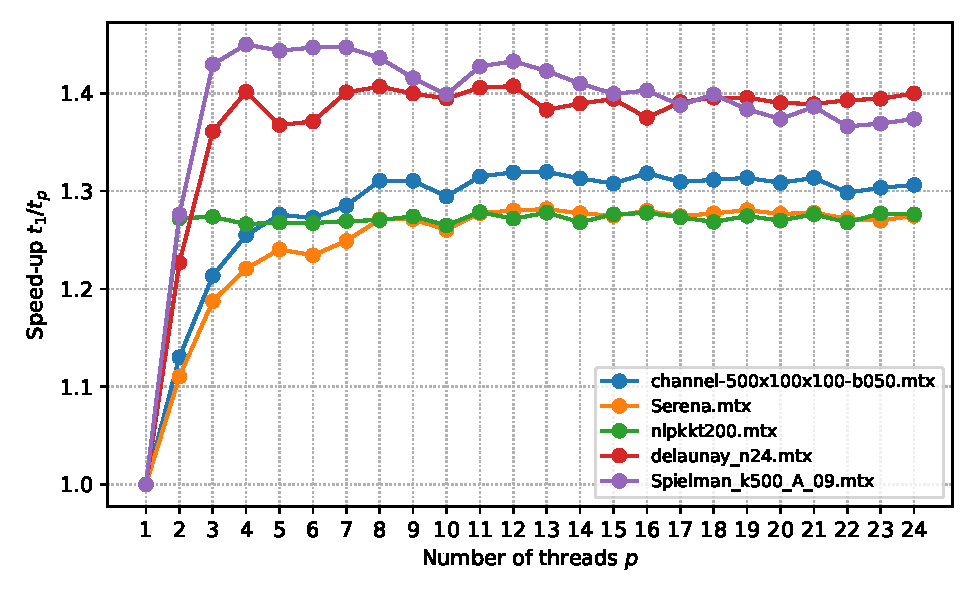
\includegraphics[width=\linewidth]{report/figures/results/speedup_t_tasks_ms_top5.pdf}
  \caption{Strong–scaling of the task-based bi-block solver
           (five largest matrices, see
           Table \ref{tab:matrices_benchmarks}), executed on the compute-p1 node of DelftBlue.}
  \label{fig:parallel_speedup_task}
\end{figure}

\begin{figure}[htb]
  \centering
  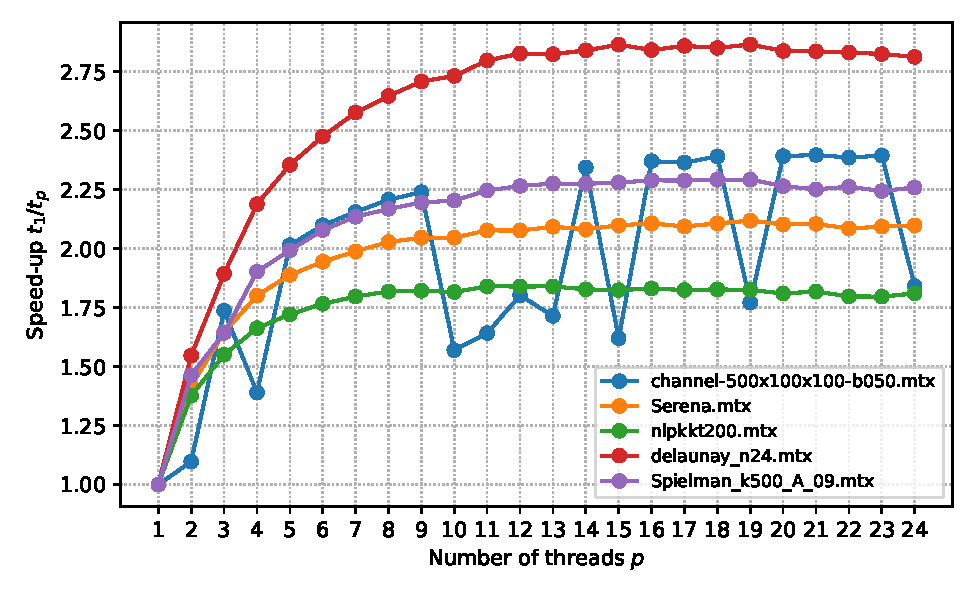
\includegraphics[width=\linewidth]{report/figures/results/speedup_t_trilinos_ms_top5.pdf}
  \caption{Strong–scaling of the Kokkos-Kernels
           \texttt{sptrsv} implementation for the same matrices and
           hardware as in Fig. \ref{fig:parallel_speedup_task}.}
  \label{fig:parallel_speedup_kokkos}
\end{figure}

For the task–graph solver
(Fig. \ref{fig:parallel_speedup_task}) the speed-up ranges from
$1.28$ ( \texttt{Serena} ) to $1.45$
( \texttt{Spielman\_k500\_A\_09.mtx} ).  
Across all cases the curve flattens once $p\gtrsim6$ because
\emph{Phase 2} (see Section \ref{chap:meth_task_sched}) becomes the critical path and thus further threads can only
steal leftover provisional tasks whose contribution to total run time
is already marginal.

Kokkos-Kernels exhibits a larger head-room
(Fig. \ref{fig:parallel_speedup_kokkos}):
$S(24)$ varies between $1.75$ and $2.8$
and saturation is only reached around $p=16$.

A notable outlier is \texttt{channel-500x100x100-b050.mtx}, whose speed-up curve alternates between two distinct plateaus, an indication that Kokkos-Kernels may toggle between two internal solve strategies for this matrix.

Intel MKL is not included in the scaling plots because
\texttt{mkl\_sparse\_trsv} is a sequential kernel
and therefore provides no meaningful parallel speed-up curve.
Its single-thread timing will be used as a performance baseline in the next sections.

%====================================================================
\subsection{Run-Time Versus Problem Size}
\label{sec:results_runtime_vs_nnz}
%--------------------------------------------------------------------
Figure \ref{fig:runtime_vs_nnz_grid} juxtaposes the
solve times of the three solvers (Intel MKL, the task–graph implementation, and the
Kokkos–Kernels reference) against the matrix size
(measured by the number of non-zeros $N_{nz}$).
Each panel fixes the thread count $p\in\{1,6,12,24\}$;
the horizontal axis is shared so that slopes can be compared
directly. All measurements were obtained on the compute-p1 node of DelftBlue (Table \ref{tab:platforms}).

At $p=1$ (upper-left panel) MKL unsurprisingly delivers the
fastest solves; its algorithmic overhead is modest and
the code is heavily optimised for serial performance.
The task solver follows the same trend
but incurs a higher constant cost because symbolic
permutation and task management are executed on the critical
path.  Kokkos–Kernels is the slowest method for most matrices, showing a larger overhead.

When additional threads become available
($p=6$, $12$, $24$) the curves of the parallel solvers turn
downwards, while the single–threaded MKL line stays in place.
For the task solver the improvement is noticeable up to
about six threads and then flattens, in line with the
strong–scaling results discussed later in
Section \ref{sec:results_speedup}.
Kokkos–Kernels continues to shorten run-time up to
$p\approx 16$ and then levels off where the turning point depends
on the matrix structure.

A final observation from Figure \ref{fig:runtime_vs_nnz_grid} is that
for small matrices ($N_{nz} \lesssim 10^{7}$) the
one-threaded Intel~MKL routine is consistently the fastest of the
three solvers even when parallel resources are available.
The higher constant overheads of the task graph (task creation) and of Kokkos-Kernels (kernel-handle initialisation,
generic data structures) outweigh their potential to exploit additional
threads.  Only when the matrix exceeds roughly ten million non-zeros does the
parallel execution of the task solver or Kokkos become beneficial
relative to MKL’s highly tuned serial path.

Because absolute run-times obscure the relative gains, and because the performance of the solvers lie very close together,
the next section converts these measurements into
speed-up curves,
which better expose algorithmic scalability.

\begin{figure}
  \centering
  \begin{subfigure}[t]{0.49\linewidth}
    \centering
    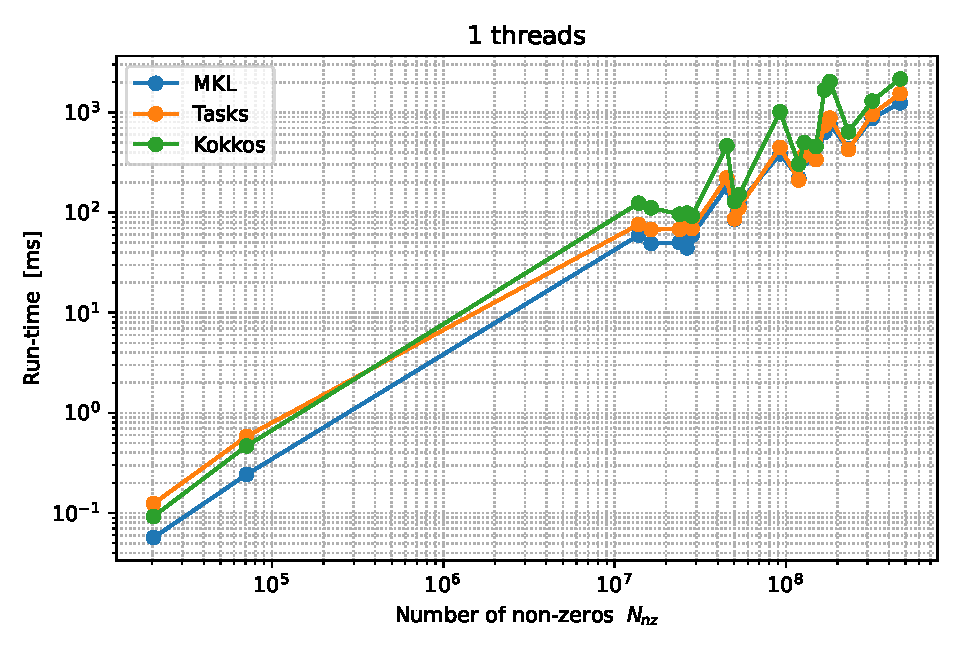
\includegraphics[width=\linewidth]{report/figures/results/runtime_vs_nnz_1.pdf}
    \caption{$p=1$ thread}
  \end{subfigure}
  %
  \begin{subfigure}[t]{0.49\linewidth}
    \centering
    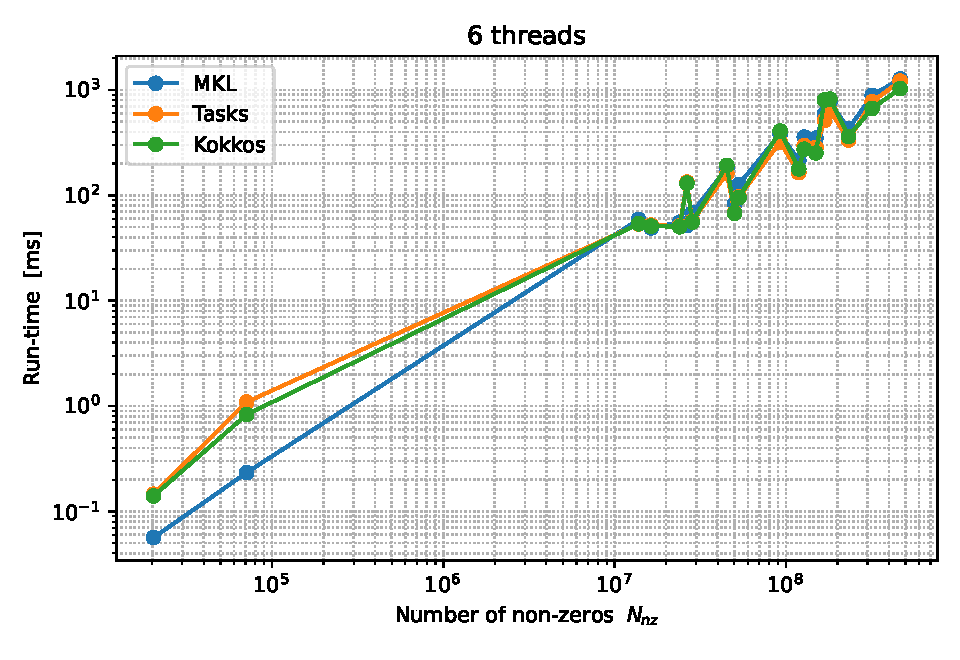
\includegraphics[width=\linewidth]{report/figures/results/runtime_vs_nnz_6.pdf}
    \caption{$p=6$ threads}
  \end{subfigure}
  \\
  \begin{subfigure}[t]{0.49\linewidth}
    \centering
    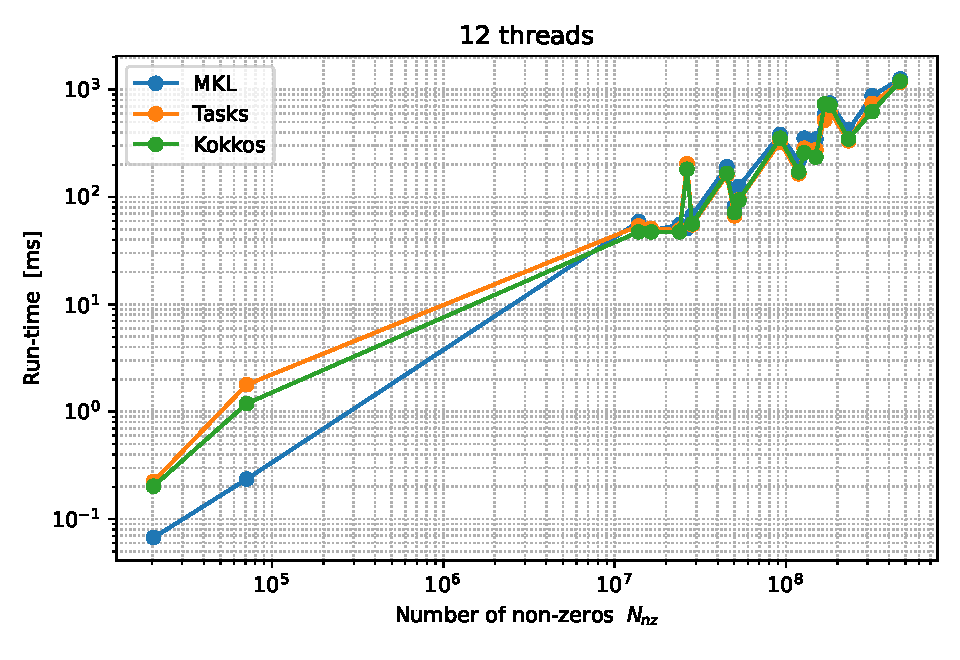
\includegraphics[width=\linewidth]{report/figures/results/runtime_vs_nnz_12.pdf}
    \caption{$p=12$ threads}
  \end{subfigure}
  %
  \begin{subfigure}[t]{0.49\linewidth}
    \centering
    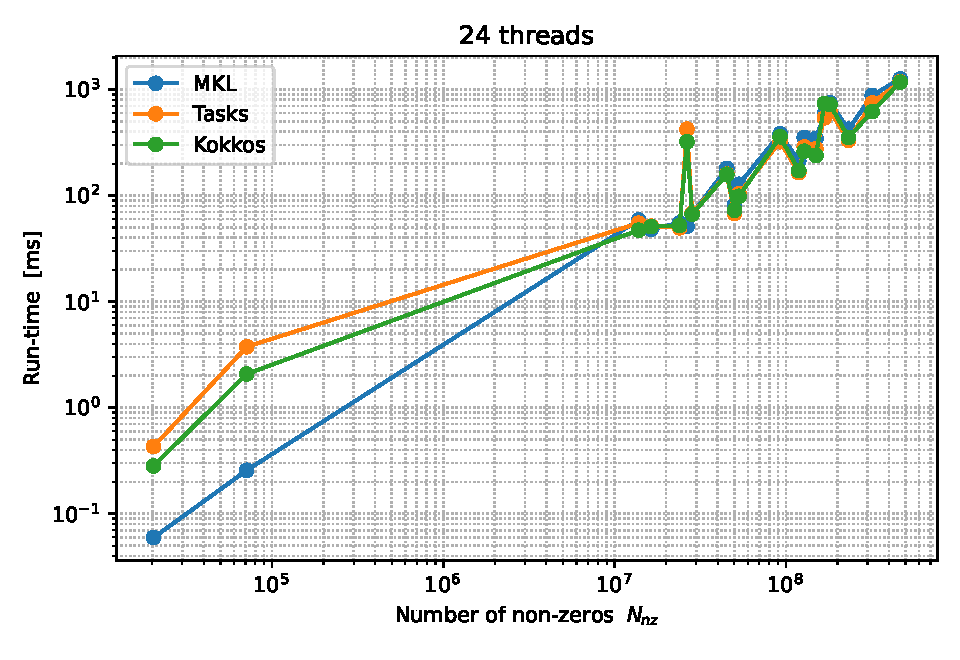
\includegraphics[width=\linewidth]{report/figures/results/runtime_vs_nnz_24.pdf}
    \caption{$p=24$ threads}
  \end{subfigure}
  \caption{Run-time versus problem size for the three solvers.
           Each line connects matrices in ascending $N_{nz}$ order and both axes use logarithmic scales. Measurements performed on the compute-p1 node of DelftBlue.}
  \label{fig:runtime_vs_nnz_grid}
\end{figure}


%====================================================================
\subsection{Cross–Solver Comparison}
\label{sec:results_rel_speedup}
%---------------------------------------------------------------
Figure \ref{fig:rel_speedup_mkl_tasks} shows the ratio
$t_{\mathrm{MKL}}/t_{\text{tasks}}$ while
Figure \ref{fig:rel_speedup_kokkos_tasks} reports
$t_{\mathrm{Kokkos}}/t_{\text{tasks}}$.
Each curve corresponds to a fixed thread count
$p\in\{1,6,12,24\}$ and is plotted over the non–zero count
of the test matrices. Measurements were once again performed on an exclusive compute-p1 node on DelftBlue (Table \ref{tab:platforms}).

Because Intel MKL’s triangular kernel is single-threaded, the ratio
$t_{\mathrm{MKL}}/t_{\text{tasks}}$ grows with $p$ making
our implementation up to an order of magnitude faster at
$p=24$.
For $p=1$ the Intel MKL solver is in almost all cases the faster method as should be expected.

In Figure \ref{fig:rel_speedup_mkl_tasks} there is one very notable outlier to the general performance trend, this turns out to be caused by matrix \texttt{Ship\_003}.
\texttt{Ship\_003} is the only test matrix that is symmetric positive-definite in its original form and therefore a direct Cholesky candidate. Its factor $L$ develops large, nearly dense super-nodes and RACE collapses these into just a few bulky diagonal blocks, leaving virtually no task-level parallelism. Our two–pass task kernel still incurs its bookkeeping overhead, but with little memory latency to overlap, this cost dominates the run time.
Conversely, \texttt{mkl\_sparse\_d\_trsv} detects the dense structure and switches to a vectorised dense micro-kernel that streams efficiently through contiguous data, even in a single thread.
Hence \texttt{Ship\_003} falls far below the general speed-up trend: MKL outperforms the task solver and additional threads cannot close the gap.
The anomaly delineates the solver’s scope: it excels on irregular, latency-dominated triangular factors, but its edge disappears when the factor resembles a dense panel already handled efficiently by a tuned serial routine.
\begin{figure}
    \centering
    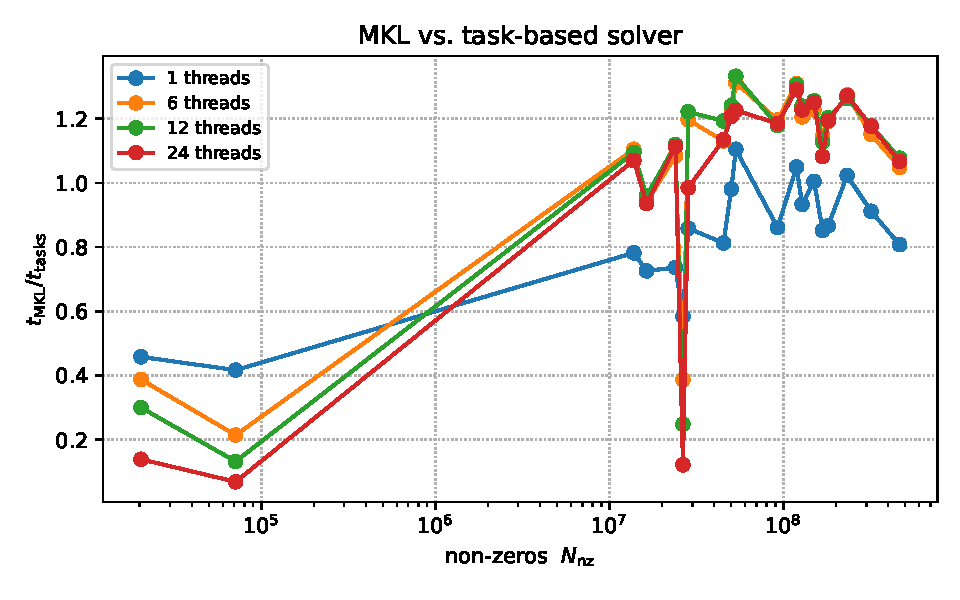
\includegraphics[width=1\linewidth]{report//figures//results/rel_speedup_mkl_vs_tasks.pdf}
    \caption{Relative speed-up $\displaystyle\frac{t_{\text{MKL}}}{t_{\text{tasks}}}$.
Points above 1 indicate that the task-based solver outperforms Intel MKL and
points below 1 indicate the opposite.  Results are shown for
$p = 1,\,6,\,12,$ and 24 threads, with matrices ordered by increasing
$\mathrm{nnz}$.}
    \label{fig:rel_speedup_mkl_tasks}
\end{figure}

The curves in Figure \ref{fig:rel_speedup_kokkos_tasks}
lie much closer to the horizontal axis,
staying between $0.75$ and $1.5$ for almost the entire size range when more then one thread is used.
This confirms that after the strong-scaling “plateau” of
Figure \ref{fig:parallel_speedup_task} is reached both
parallel algorithms become memory-bound and therefore deliver
very similar absolute performance.
The apparent advantage of Kokkos at $p\ge 12$ must therefore be read
with caution: it reflects the fact that our method saturates a few
threads earlier and subsequently shows little change, whereas the
Kokkos implementation continues to shorten its run time until about
$p\approx16{-}18$.
When the arithmetic workload is tiny (leftmost data points) the Kokkos
solver is clearly faster for $p \geq1$.

\begin{figure}
    \centering
    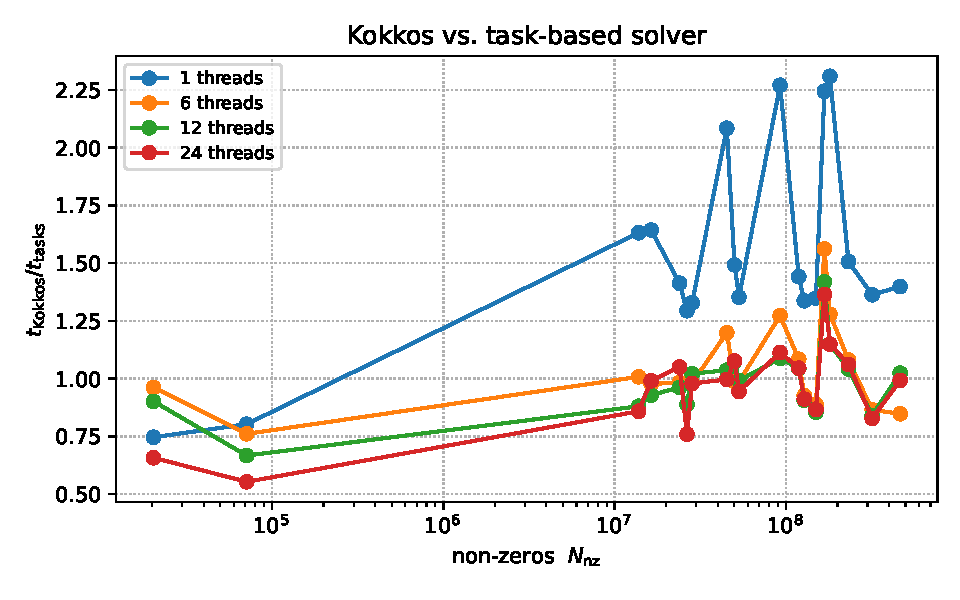
\includegraphics[width=1\linewidth]{report//figures//results/rel_speedup_kokkos_vs_tasks.pdf}
    \caption{Relative speed-up $\displaystyle\frac{t_{\text{Kokkos}}}{t_{\text{tasks}}}$.
Values above 1 mean the task-based solver is faster than the Kokkos-Kernels
implementation, while values below 1 favour Kokkos.}
    \label{fig:rel_speedup_kokkos_tasks}
\end{figure}

The two ratios underline that speed-up is a relative metric:
although Kokkos attains larger strong-scaling factors
(Figure \ref{fig:parallel_speedup_kokkos}),
its advantage in wall-clock time shrinks once both solvers are limited
by memory bandwidth.
Put differently, the task‐graph formulation reaches the memory-bound
regime earlier, so its speed-up curve becomes flat
before Kokkos has exhausted all available cores.
For large matrices and $p\ge12$ the two implementations therefore
exhibit virtually identical run times.

Across the large-matrix test set no single solver dominates
universally: for some inputs the task-based bi-block method is faster,
for others the Kokkos implementation wins.
The relative ranking therefore depends on the individual sparsity
pattern rather than on matrix size alone.

%---------------------------------------------------------------------------
\subsection{LIKWID Results}
\label{sec:results:cache-reuse}
All LIKWID measurements were taken on the DelftBlue compute-p2 node (\ref{tab:platforms}).
The region of our solver was instrumented with the \textit{L3}, \textit{L2/L2CACHE}
and \textit{DATA} event groups.
The \textit{MEM} group is unavailable on this
platform because current LIKWID versions cannot program the Intel Sapphire Rapids
integrated-memory-controller, so the counters \texttt{CAS\_COUNT\_RD/WR}
return 0. Consequently, the analysis below focuses on the on-chip hierarchy only.

LIKWID was used to measure the difference in performance of the task-based model implemented with OpenMP in Section \ref{sec:impl_tasks}, before the affinity clause was added to the OpenMP directives. 
To interpret the cache behaviour we restrict the discussion to a single
matrix that cannot reside in any on-chip cache and therefore
stresses the reuse mechanisms most: \texttt{nlpkkt200} (see Table \ref{tab:matrices_benchmarks}).
After the $A^3$ expansion and triangular extraction the factor
is sure to not fit in the cache memory of \textit{DelftBlue}.


With the LIKWID \texttt{L3}, \texttt{L2CACHE} and \texttt{DATA} groups
the triangular solve of our task kernel (16 threads) reports

$$
\mathrm{L3\;loads}=7.1\;\text{GB}, \quad
\mathrm{L3\;miss\;ratio}=12\%, \qquad
\mathrm{L2\;miss\;ratio}=91\%.
$$

The missing \texttt{MEM} group on Sapphire Rapids prevents
direct DRAM-traffic measurements; nonetheless the figures are
consistent with an in-LLC working set.
Almost every line requested by a core is absent from its private L2,
but nine out of ten are satisfied in the shared LLC, so only
$\approx 0.85\;\text{GB}$ of the 7.1 GB finally spill to memory.

A {\small $\sim$90 \%} L2 miss rate means that most provisional and
correction tasks run on different cores:
the provisional pass of block~$i$ brings
$L_i$ and $x_i$ into its private cache, the correction pass is then stolen by
another worker, and the data are fetched again from LLC.
This behaviour confirms the suspicion that the default
work-stealing policy weakens the intended producer–consumer affinity.
When the same thread executed both phases in quick succession one would
expect up to 50 \% L2 hits, because an entire $L_i$ ($\le$2 MiB)
fits into a single private cache.

In Section~\ref{sec:impl_tasks_aff} the \texttt{affinity} clause was
added to the OpenMP task directives to keep each correction task on the
same core that had just produced its matching provisional result,
thereby preserving the block data in the private~L2 cache.  Owing to
time constraints in the final week of the project, a second LIKWID
counter study could not be performed; only wall-clock timings were
recorded.

Those timings are nevertheless decisive.  For every matrix and for all
thread counts $p\in\{1,2,3,6,9,12\}$ the version with the
\texttt{affinity} hint outperforms the earlier non-affine
implementation.  Figure~\ref{fig:speedup_non_aff_aff} plots the ratio
$$
  \text{speed-up}_{\mathrm{aff}}=\frac{t_{\text{no-affinity}}}{t_{\text{affinity}}},
$$
so values above $1$ indicate a benefit from affinity scheduling.  The
average improvement ranges from $\sim1.1\times$ for single-thread
runs—where no scheduling decisions are necessary—up to almost
$\sim2 \times$ for nine threads.  This confirms the intuition from
Section \ref{sec:impl_tasks_aff}: suppressing work-stealing along the
tightly coupled correction chain leads to markedly better cache-line
reuse and shorter overall solve time, even though the
\texttt{affinity} clause is merely a hint and the OpenMP runtime may, in
principle, choose a different mapping.
\begin{figure}
    \centering
    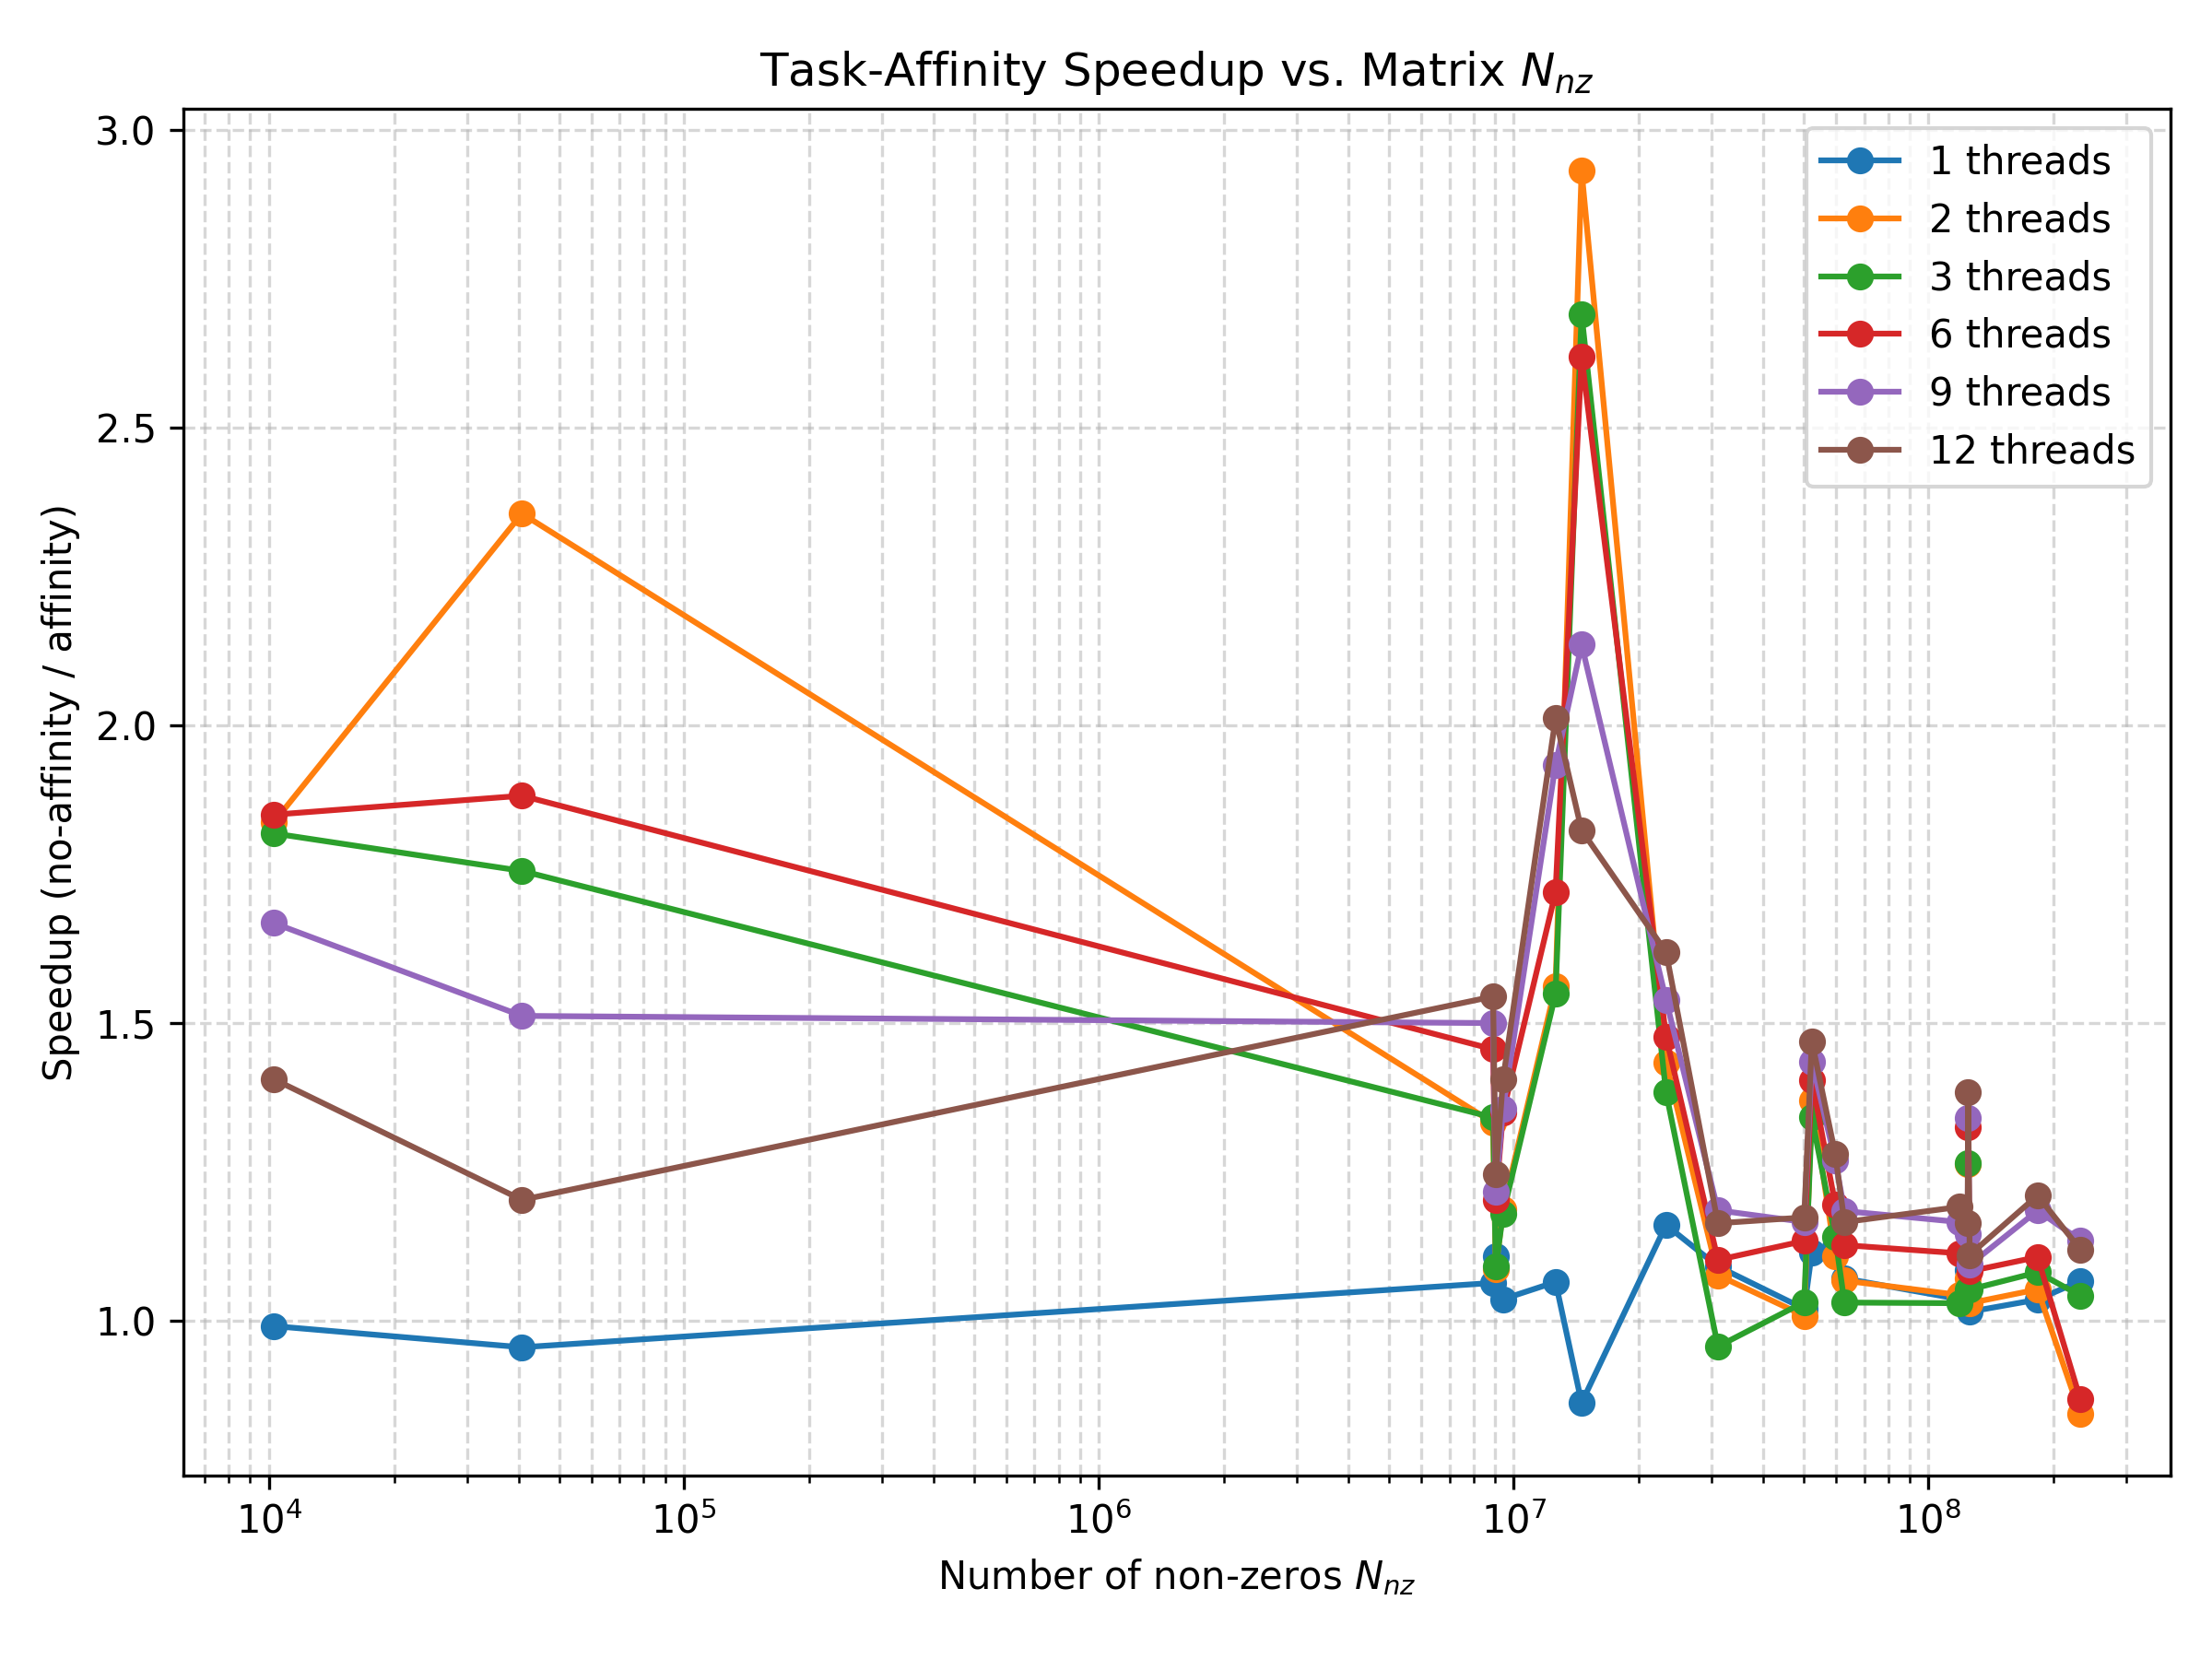
\includegraphics[width=1\linewidth]{relative_speedup_affinity_non_aff.png}
    \caption{Relative speed-up between the task based solver when implemented with and without affinity clause. Speed-up is given by solve time of implementation without affinity divided by the implementation with affinity for p $\in \{1,2,3,6,9,12 \}$ threads.}
    \label{fig:speedup_non_aff_aff}
\end{figure}
%---------------------------------------------------------------------------

\section{Reproducibility and Data Availability}
\label{sec:results_data}
All raw CSV measurements, plotting scripts, and the exact solver
sources that produced the figures of this chapter are publicly
available at \url{https://github.com/IdsRehorst/Bachelor-Thesis-Ids-Rehorst}.
The repository’s \texttt{tests/} directory contains
\texttt{benchmark\_\(<p>\).csv} files – one per thread count – that hold  
the median run time of every matrix and solver variant,  
ready for independent analysis or alternative visualisations.
 

\chapter{Conclusion}
\label{chapter:conclusion}

\emph{A conclusion...}


%% Prevent urls running into margins in bibliography
\setcounter{biburlnumpenalty}{7000}
\setcounter{biburllcpenalty}{7000}
\setcounter{biburlucpenalty}{7000}

%% Add bibliography
\printbibliography[heading=bibintoc,title=References]

%% ----------------------------------------------------------------------
%%    Appendix (Letters for chapters)
%% ----------------------------------------------------------------------
\appendix

\chapter{Source Code Example}
%\label{chapter:title}

\emph{Adding source code to your report/thesis is supported with the package {\normalfont\texttt{listings}}. An example can be found below. Files can be added using {\normalfont\texttt{\textbackslash lstinputlisting[language=<language>]\{<filename>\}}}.}

\begin{lstlisting}[language=Python]
"""
ISA Calculator: import the function, specify the height and it will return a
list in the following format: [Temperature,Density,Pressure,Speed of Sound].
Note that there is no check to see if the maximum altitude is reached.
"""

import math
g0 = 9.80665
R = 287.0
layer1 = [0, 288.15, 101325.0]
alt = [0,11000,20000,32000,47000,51000,71000,86000]
a = [-.0065,0,.0010,.0028,0,-.0028,-.0020]

def atmosphere(h):
    for i in range(0,len(alt)-1):
        if h >= alt[i]:
            layer0 = layer1[:]
            layer1[0] = min(h,alt[i+1])
            if a[i] != 0:
                layer1[1] = layer0[1] + a[i]*(layer1[0]-layer0[0])
                layer1[2] = layer0[2] * (layer1[1]/layer0[1])**(-g0/(a[i]*R))
            else:
                layer1[2] = layer0[2]*math.exp((-g0/(R*layer1[1]))*(layer1[0]-layer0[0]))
    return [layer1[1],layer1[2]/(R*layer1[1]),layer1[2],math.sqrt(1.4*R*layer1[1])]
\end{lstlisting}

\chapter{Task Division Example}
%\label{chapter:title}

\emph{If a task division is required, a simple template can be found below for convenience. Feel free to use, adapt or completely remove.}

\begin{table}[htb]
    \setlength\extrarowheight{4pt}
    \centering
    \caption{Distribution of the workload}
    \label{tab:taskdivision}
    \begin{tabularx}{\textwidth}{lXX}
        \toprule
        & Task & Student Name(s) \\
        \midrule
        & Summary & \\
        Chapter 1 & Introduction &  \\
        Chapter 2 &  & \\
        Chapter 3 &  & \\
        Chapter * &  & \\
        Chapter * & Conclusion &  \\
        \midrule
        & Editors & \\
        & CAD and Figures & \\
        & Document Design and Layout & \\
        \bottomrule
    \end{tabularx}
\end{table}

\chapter{SpTRSV Implementation with Intel MKL}
\label{app:code_mkl}
The full implementation of the Intel MKL based solver used as a reference to the method presented in Appendix \ref{app:code} is given below.
\begin{lstlisting}[language=C++,caption={Full implementation of the
\texttt{MKL SpTRSV} kernel.}]
    void solver::mklTriSolve(const sparsemat &B, bool lower,
                         const std::vector<double> &b,
                         std::vector<double> &x)
{
    int n = B.n;

    // --- check if every row has an explicit diagonal --------------------
    bool explicitDiag = true;
    for (int r = 0; r < n && explicitDiag; ++r) {
        bool found = false;
        for (int p = B.rowPtr[r]; p < B.rowPtr[r + 1]; ++p)
            if (B.col[p] == r) { found = true; break; }
        explicitDiag = found;
    }


    sparse_matrix_t A = nullptr;
    matrix_descr desc{};
    desc.type = SPARSE_MATRIX_TYPE_TRIANGULAR;
    desc.mode = lower ? SPARSE_FILL_MODE_LOWER : SPARSE_FILL_MODE_UPPER;
    desc.diag = explicitDiag ? SPARSE_DIAG_NON_UNIT : SPARSE_DIAG_UNIT;

    std::vector<MKL_INT> ia(n + 1);  std::vector<MKL_INT> ja(B.col.size());
    for (int i = 0; i <= n; ++i) ia[i] = B.rowPtr[i];
    for (size_t k = 0; k < B.col.size(); ++k) ja[k] = B.col[k];

    // Init Likwid marker for measuring perfomance
    LIKWID_MARKER_START("MKL");

    mkl_sparse_d_create_csr(&A, SPARSE_INDEX_BASE_ZERO,
                            n, n, ia.data(), ia.data() + 1,
                            ja.data(), const_cast<double*>(B.val.data()));
    mkl_sparse_optimize(A);

    x.assign(n, 0.0);
    mkl_sparse_d_trsv(SPARSE_OPERATION_NON_TRANSPOSE,
                      1.0, A, desc,
                      b.data(), x.data());
    mkl_sparse_destroy(A);
    LIKWID_MARKER_STOP("MKL");
}
\end{lstlisting}


\end{document}
